\documentclass[a4paper,16pt]{article}
\usepackage{cite}
\usepackage{url}
\usepackage{amsmath,amssymb}
\usepackage{lipsum}
\usepackage[dvipdfmx]{graphicx}


\bibliographystyle{ieice}

\author{sXXXXXXX - Taro Aizu (sXXXXXXX@u-aizu.ac.jp)}
\title{Homework 1 \\ ...............................................................................................\\CSANN Lecture title  \\ {\large by Prof. John Doe}}


\setlength{\textheight}{\paperheight}   % 紙面縦幅を本文領域にする(BOTTOM=-TOP)
\addtolength{\topmargin}{-\headsep}     % ヘッダの分だけ本文領域を移動させる
\addtolength{\textheight}{-60truemm}    % 下の余白も30mm(BOTTOM=-TOPだから+TOP+30mm)

\setlength{\textwidth}{\paperwidth}     % 紙面横幅を本文領域にする(RIGHT=-LEFT)
\setlength{\oddsidemargin}{-0.4truemm}  % 左の余白を25mm(=1inch-0.4mm)に
\setlength{\evensidemargin}{-0.4truemm} % 
\addtolength{\textwidth}{-50truemm}     % 右の余白も25mm(RIGHT=-LEFT)


\begin{document}
\maketitle


\section*{Lecture N Exercise}
{\bf Problem:} \\
See Figure \ref{graph:other}
\footnote{http://hyoushiki.graph.jp/2keikai/keikai215.html}

\begin{figure}[htbp!]
 \begin{center}
  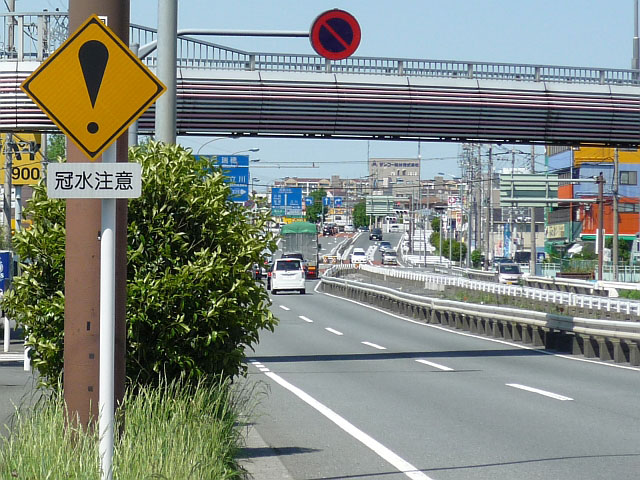
\includegraphics[width=9cm, height=7cm]{./img/image.jpg}
  \caption{Caption}
  \label{graph:other}
 \end{center}
\end{figure}

\begin{itemize}
  \item 1
  \item[2.] test
\end{itemize}

Let $N = 1$, then

\begin{eqnarray*}
  N + N = 2
\end{eqnarray*}


\end{document}